% Preamble
\documentclass[conference]{IEEEtran}
% Some Computer Society conferences also require the compsoc mode option,
% but others use the standard conference format.
%
% If IEEEtran.cls has not been installed into the LaTeX system files,
% manually specify the path to it like:
% \documentclass[conference]{../sty/IEEEtran}
\usepackage[brazilian]{babel}
\usepackage[utf8]{inputenc}
\usepackage[T1]{fontenc}
\usepackage{amsmath}
\usepackage{algorithm}
\usepackage[]{algpseudocode}
\usepackage{graphicx}
\usepackage{caption}

\makeatletter
\renewcommand{\ALG@name}{Algoritmo}
\def\BState{\State\hskip-\ALG@thistlm}
\makeatother

% Some very useful LaTeX packages include:
% (uncomment the ones you want to load)


% *** MISC UTILITY PACKAGES ***
%
%\usepackage{ifpdf}
% Heiko Oberdiek's ifpdf.sty is very useful if you need conditional
% compilation based on whether the output is pdf or dvi.
% usage:
% \ifpdf
%   % pdf code
% \else
%   % dvi code
% \fi
% The latest version of ifpdf.sty can be obtained from:
% http://www.ctan.org/pkg/ifpdf
% Also, note that IEEEtran.cls V1.7 and later provides a builtin
% \ifCLASSINFOpdf conditional that works the same way.
% When switching from latex to pdflatex and vice-versa, the compiler may
% have to be run twice to clear warning/error messages.






% *** CITATION PACKAGES ***
%
%\usepackage{cite}
% cite.sty was written by Donald Arseneau
% V1.6 and later of IEEEtran pre-defines the format of the cite.sty package
% \cite{} output to follow that of the IEEE. Loading the cite package will
% result in citation numbers being automatically sorted and properly
% "compressed/ranged". e.g., [1], [9], [2], [7], [5], [6] without using
% cite.sty will become [1], [2], [5]--[7], [9] using cite.sty. cite.sty's
% \cite will automatically add leading space, if needed. Use cite.sty's
% noadjust option (cite.sty V3.8 and later) if you want to turn this off
% such as if a citation ever needs to be enclosed in parenthesis.
% cite.sty is already installed on most LaTeX systems. Be sure and use
% version 5.0 (2009-03-20) and later if using hyperref.sty.
% The latest version can be obtained at:
% http://www.ctan.org/pkg/cite
% The documentation is contained in the cite.sty file itself.






% *** GRAPHICS RELATED PACKAGES ***
%
\ifCLASSINFOpdf
  % \usepackage[pdftex]{graphicx}
  % declare the path(s) where your graphic files are
  % \graphicspath{{../pdf/}{../jpeg/}}
  % and their extensions so you won't have to specify these with
  % every instance of \includegraphics
  % \DeclareGraphicsExtensions{.pdf,.jpeg,.png}
\else
  % or other class option (dvipsone, dvipdf, if not using dvips). graphicx
  % will default to the driver specified in the system graphics.cfg if no
  % driver is specified.
  % \usepackage[dvips]{graphicx}
  % declare the path(s) where your graphic files are
  % \graphicspath{{../eps/}}
  % and their extensions so you won't have to specify these with
  % every instance of \includegraphics
  % \DeclareGraphicsExtensions{.eps}
\fi
% graphicx was written by David Carlisle and Sebastian Rahtz. It is
% required if you want graphics, photos, etc. graphicx.sty is already
% installed on most LaTeX systems. The latest version and documentation
% can be obtained at: 
% http://www.ctan.org/pkg/graphicx
% Another good source of documentation is "Using Imported Graphics in
% LaTeX2e" by Keith Reckdahl which can be found at:
% http://www.ctan.org/pkg/epslatex
%
% latex, and pdflatex in dvi mode, support graphics in encapsulated
% postscript (.eps) format. pdflatex in pdf mode supports graphics
% in .pdf, .jpeg, .png and .mps (metapost) formats. Users should ensure
% that all non-photo figures use a vector format (.eps, .pdf, .mps) and
% not a bitmapped formats (.jpeg, .png). The IEEE frowns on bitmapped formats
% which can result in "jaggedy"/blurry rendering of lines and letters as
% well as large increases in file sizes.
%
% You can find documentation about the pdfTeX application at:
% http://www.tug.org/applications/pdftex





% *** MATH PACKAGES ***
%
%\usepackage{amsmath}
% A popular package from the American Mathematical Society that provides
% many useful and powerful commands for dealing with mathematics.
%
% Note that the amsmath package sets \interdisplaylinepenalty to 10000
% thus preventing page breaks from occurring within multiline equations. Use:
%\interdisplaylinepenalty=2500
% after loading amsmath to restore such page breaks as IEEEtran.cls normally
% does. amsmath.sty is already installed on most LaTeX systems. The latest
% version and documentation can be obtained at:
% http://www.ctan.org/pkg/amsmath





% *** SPECIALIZED LIST PACKAGES ***
%
%\usepackage{algorithmic}
% algorithmic.sty was written by Peter Williams and Rogerio Brito.
% This package provides an algorithmic environment fo describing algorithms.
% You can use the algorithmic environment in-text or within a figure
% environment to provide for a floating algorithm. Do NOT use the algorithm
% floating environment provided by algorithm.sty (by the same authors) or
% algorithm2e.sty (by Christophe Fiorio) as the IEEE does not use dedicated
% algorithm float types and packages that provide these will not provide
% correct IEEE style captions. The latest version and documentation of
% algorithmic.sty can be obtained at:
% http://www.ctan.org/pkg/algorithms
% Also of interest may be the (relatively newer and more customizable)
% algorithmicx.sty package by Szasz Janos:
% http://www.ctan.org/pkg/algorithmicx




% *** ALIGNMENT PACKAGES ***
%
%\usepackage{array}
% Frank Mittelbach's and David Carlisle's array.sty patches and improves
% the standard LaTeX2e array and tabular environments to provide better
% appearance and additional user controls. As the default LaTeX2e table
% generation code is lacking to the point of almost being broken with
% respect to the quality of the end results, all users are strongly
% advised to use an enhanced (at the very least that provided by array.sty)
% set of table tools. array.sty is already installed on most systems. The
% latest version and documentation can be obtained at:
% http://www.ctan.org/pkg/array


% IEEEtran contains the IEEEeqnarray family of commands that can be used to
% generate multiline equations as well as matrices, tables, etc., of high
% quality.




% *** SUBFIGURE PACKAGES ***
%\ifCLASSOPTIONcompsoc
%  \usepackage[caption=false,font=normalsize,labelfont=sf,textfont=sf]{subfig}
%\else
%  \usepackage[caption=false,font=footnotesize]{subfig}
%\fi
% subfig.sty, written by Steven Douglas Cochran, is the modern replacement
% for subfigure.sty, the latter of which is no longer maintained and is
% incompatible with some LaTeX packages including fixltx2e. However,
% subfig.sty requires and automatically loads Axel Sommerfeldt's caption.sty
% which will override IEEEtran.cls' handling of captions and this will result
% in non-IEEE style figure/table captions. To prevent this problem, be sure
% and invoke subfig.sty's "caption=false" package option (available since
% subfig.sty version 1.3, 2005/06/28) as this is will preserve IEEEtran.cls
% handling of captions.
% Note that the Computer Society format requires a larger sans serif font
% than the serif footnote size font used in traditional IEEE formatting
% and thus the need to invoke different subfig.sty package options depending
% on whether compsoc mode has been enabled.
%
% The latest version and documentation of subfig.sty can be obtained at:
% http://www.ctan.org/pkg/subfig




% *** FLOAT PACKAGES ***
%
%\usepackage{fixltx2e}
% fixltx2e, the successor to the earlier fix2col.sty, was written by
% Frank Mittelbach and David Carlisle. This package corrects a few problems
% in the LaTeX2e kernel, the most notable of which is that in current
% LaTeX2e releases, the ordering of single and double column floats is not
% guaranteed to be preserved. Thus, an unpatched LaTeX2e can allow a
% single column figure to be placed prior to an earlier double column
% figure.
% Be aware that LaTeX2e kernels dated 2015 and later have fixltx2e.sty's
% corrections already built into the system in which case a warning will
% be issued if an attempt is made to load fixltx2e.sty as it is no longer
% needed.
% The latest version and documentation can be found at:
% http://www.ctan.org/pkg/fixltx2e


%\usepackage{stfloats}
% stfloats.sty was written by Sigitas Tolusis. This package gives LaTeX2e
% the ability to do double column floats at the bottom of the page as well
% as the top. (e.g., "\begin{figure*}[!b]" is not normally possible in
% LaTeX2e). It also provides a command:
%\fnbelowfloat
% to enable the placement of footnotes below bottom floats (the standard
% LaTeX2e kernel puts them above bottom floats). This is an invasive package
% which rewrites many portions of the LaTeX2e float routines. It may not work
% with other packages that modify the LaTeX2e float routines. The latest
% version and documentation can be obtained at:
% http://www.ctan.org/pkg/stfloats
% Do not use the stfloats baselinefloat ability as the IEEE does not allow
% \baselineskip to stretch. Authors submitting work to the IEEE should note
% that the IEEE rarely uses double column equations and that authors should try
% to avoid such use. Do not be tempted to use the cuted.sty or midfloat.sty
% packages (also by Sigitas Tolusis) as the IEEE does not format its papers in
% such ways.
% Do not attempt to use stfloats with fixltx2e as they are incompatible.
% Instead, use Morten Hogholm'a dblfloatfix which combines the features
% of both fixltx2e and stfloats:
%
% \usepackage{dblfloatfix}
% The latest version can be found at:
% http://www.ctan.org/pkg/dblfloatfix




% *** PDF, URL AND HYPERLINK PACKAGES ***
%
%\usepackage{url}
% url.sty was written by Donald Arseneau. It provides better support for
% handling and breaking URLs. url.sty is already installed on most LaTeX
% systems. The latest version and documentation can be obtained at:
% http://www.ctan.org/pkg/url
% Basically, \url{my_url_here}.




% *** Do not adjust lengths that control margins, column widths, etc. ***
% *** Do not use packages that alter fonts (such as pslatex).         ***
% There should be no need to do such things with IEEEtran.cls V1.6 and later.
% (Unless specifically asked to do so by the journal or conference you plan
% to submit to, of course. )


% correct bad hyphenation here
\hyphenation{op-tical net-works semi-conduc-tor}

\begin{document}

% Document header
%
% paper title
% Titles are generally capitalized except for words such as a, an, and, as,
% at, but, by, for, in, nor, of, on, or, the, to and up, which are usually
% not capitalized unless they are the first or last word of the title.
% Linebreaks \\ can be used within to get better formatting as desired.
% Do not put math or special symbols in the title.
\title{Relatório 2 - ELE-32\\ Códigos de Bloco Cíclicos e BCH}


% author names and affiliations
% use a multiple column layout for up to three different
% affiliations
\author{\IEEEauthorblockN{Aloysio Galvão Lopes}
\IEEEauthorblockA{Departamento de\\Engenharia da Computação\\
Instituto Tecnológico de Aeronáutica\\
São José dos Campos, São Paulo\\
Email: aloysiogl@gmail.com}
\and
\IEEEauthorblockN{Vitor Pimenta dos Reis Arruda}
\IEEEauthorblockA{Departamento de\\Engenharia da Computação\\
Instituto Tecnológico de Aeronáutica\\
São José dos Campos, São Paulo\\
Email: vitor\_pimenta97@hotmail.com}}

\maketitle

% As a general rule, do not put math, special symbols or citations
% in the abstract
\begin{abstract}

Colocar o resumo

\end{abstract}

% no keywords

\IEEEpeerreviewmaketitle

% Ideia: 
% - Introdução resume o que fizemos: Implementamos códigos
%	cíclicos e BCH
% - Seção cobre códigos cíclicos explica como foram decodificados
%	(detalha melhor o algoritmo que está mal escrito no roteiro do Manish)
% - Seção sobre BCH explica o que ele é e seu algoritmo de decodificação
%	(acho que vou é colocar a referência e fim de papo)
% - Seção "Resultados" mostra os gráficos de chance de erro para mostrar
%	quem é quem e o gráfico de complexidade do BCH para validar que ele
%	é linear no tamanho do bloco
%

\section{Código convolucionais}

Os códigos convolucionais baseiam-se na convolução de um sinal de entrada com um sistema codificador. Um codificador convolucional pode ser interpretado como uma máquina de estados que processa $k$ bits de entrada gerando $n>k$ bits de saída de forma que cada conjunto de bits gerados dependam do bit de processado e do estado atual da máquina.

O processo de codificação consiste em realizar o processamento dos bits pela máquina de estado, a cada iteração é alterado o estado da máquina e os bits de saída são processados de acordo com os polinômios geradores descrito pela máquina. No processo de decodificação é utilizado o algoritmo de Viterbi, que consiste em encontrar a sequencia de entrada da máquina que melhor aproxima a sequencia  de decodificação.

\section{Comparação Justa}
Nas práticas anteriores, para comparar a eficácia dos códigos utilizados, montavam-se gráficos da probabilidade de erro (eixo y) pela probabilidade de erro de bit no canal (eixo x) em escala logarítmica. Embora essa comparação forneça uma noção  a respeito da melhora obtida por um determinado código, a comparação não leva em conta que a introdução de redundância aumenta a energia que é utilizada para transmitir um bit de informação.

Poderíamos apenas aumentar a energia de uma codificação considerada menos eficiente anteriormente e ela teria probabilidade de erro menor. Dessa forma, a comparação justa deveria supor mesmo $\frac{E_i}{N_0}$. Supondo uma modulação BPSK, $p\left(\frac{E_b}{N_0}\right) = Q\left(\sqrt{\frac{E_b}{N_0}}\right)$. Dessa forma, considerando mesmo $\frac{E_i}{N_0}$, tem-se $p\left(\frac{E_i}{N_0}\right) = Q\left(\sqrt{\frac{E_i}{N_0}\frac{k}{n}}\right)$.

Os valores de $p$ utilizados nos experimentos anteriores foram remapeados supondo $k = n$. Dessa forma, obtiveram-se valores de $\frac{E_i}{N_0}$ para serem utilizados para cada tipo de codificação. Ressalta-se que tais valores foram muito parecidos com uma sequência de 0 a 10 igualmente espaçada. Os valores são apresentados abaixo.

0.1, 0.35416315, 0.82118721, 1.35277173, 2.10894229, 2.70594722,
	3.3174483, 4.1419075, 4.77476785, 5.41378309, 6.26609665, 6.91554181,
	7.56835261, 8.43569456, 9.09464674, 9.75571048, 10.63242365.
	
Antes de realizar a codificação essa sequência de valores passa pela função \textit{p\_map(k,n)}, a qual gera a sequência de probabilidades de erro correspondentes a um código de taxa dada por $k$ e $n$. Essa função realiza a operação $p\left(\frac{E_i}{N_0}\right) = Q\left(\sqrt{\frac{E_i}{N_0}\frac{k}{n}}\right)$ em cada um dos valores do vetor de $\frac{E_i}{N_0}$ acima. Desse modo, pode-se reutilizar exatamente o mesmo código das práticas anteriores apenas com um remapeamento dos valores de $p$.

Todos os gráficos gerados nesse relatório utilizam o método de comparação aqui descrito.

\section{Algoritmos para códigos convolucionais}
A algoritmo desenvolvido pode ser dividido nas seguintes etapas: codificação, e decodificação. Cada uma dessas etapas esta descrita nas subseções seguintes.

\subsection{Codificação}

% DIFICULDADES PARA IMPLMENTAR CODIFICADOR

A codificação consistiu processar os bits de entrada pela máquina de estado descrita pelos polinômios geradores fornecidos, descritos pela Tabela \ref{tab:polinomios_geradores}. $m$ indica a quantidade de memórias da máquina, e, consequentemente, o número de estados que ela pode atingir.

\begin{table}[h!]
	\centering
	\caption{Polinômios geradores na forma octal}
	\label{tab:polinomios_geradores}
	\begin{tabular}{|c|c|c|c|}
		\hline
		$m$ & $g1(D)$ & $g2(D)$ & $g3(D)$ \\ \hline\hline
		 3  &   13    &   15    &   17    \\ \hline
		 4  &   25    &   33    &   37    \\ \hline
		 6  &   117   &   127   &   155   \\ \hline
	\end{tabular} 
\end{table}

Partindo do estado nulo, o processamento da máquina consiste em dado um bit, gerar 3 bits codificados de acordo com o valor armazenado nas $m$ memórias e os polinômios geradores, deslocar o valor das memórias, e então o bit recebido passa a ocupar a primeira memória. Dessa forma, o código possui taxa $1/3$.

%Sendo $G(D)$ uma matriz cujas linhas representam os polinômios geradores e $u(D)$ a mensagem a ser transmitida. Matematicamente, a mensagem codificada, $v(D)$, pode ser interpretado como descrito em (\ref{eq:mensagem_codificada}).
%
%\begin{equation}
%	s(D) = u(D).G(D)
%\end{equation}
%
%\begin{equation}
%	v(D) = \sum_{i=1}^{n} s_{i}(D^{n})D^{i-1}
%	\label{eq:mensagem_codificada}
%\end{equation}


\subsection{Decodificação}

Nesta parte do experimento é necessário utilizar o algoritmo de Viterbi para realizar a decodificação do código gerado. A ideia por trás desse algoritmo é armazenar os custos dos caminhos possíveis, a partir do estado nulo, de acordo com a mensagem transmitida. O custo de um caminho é obtido pela soma dos custos dos ramos que formam o percurso.

Para evitar, crescer exponencialmente com as possibilidades de percursos, o algoritmo de Viterbi aproveita-se do fato que vários percursos levam a um mesmo estado. Assim, pode-se escolher apenas o percurso mais provável para aquele estado um instante de tempo. Como critério é usado que o caminho mais provável é o com menor custo, pois está sendo adotado que o canal tem maior taxa de acerto.

Para decidir a sequencia correta que foi transmitida foi implementado o algoritmo de Viterbi já descrito. O pseudocódigo para tal algoritmo é mostrado em Algoritmo \ref{alg:viterbi}.

\begin{algorithm}[h!]
	\caption{Decodificação}
	\label{alg:viterbi}
	\begin{algorithmic}[Message]		
		\Procedure{$decode$}{$message$}
			\State $Custo[0] \gets 0$
			\State $Custo[i] \gets \infty, \forall i \ne 0$
			
			\For {$simb \in message$}
				\For {$Estados futuro - f$}
					\State $Custo[f] \gets min(Custo[i] + trans(i, f, simb))$
				\EndFor
			\EndFor
			
			\State {$x \gets min(Custo)$}					
			
		\Return $caminho[x]$
		\EndProcedure
	\end{algorithmic}
\end{algorithm}

Para calcular o custo de determinada transição é usado a distância de Hamming entre o simbolo recebido e o simbolo associado à transição. O Algoritmo \ref{alg:hamming} apresenta o pseudocódigo para esse caso.

\begin{algorithm}[h!]
	\caption{Distância de Hamming}
	\label{alg:hamming}
	\begin{algorithmic}[Message]		
		\Procedure{$hamming$}{$inicial$, $final$, $simb$}
		\State $esperado \gets simbolo(inicial, final)$
		\State $custo = 0$
		
		\For {$i \in len(simb)$}
			\State $custo += simb[i] + esperado[i] \% 2$
		\EndFor
		
		\Return $custo$
		\EndProcedure
	\end{algorithmic}
\end{algorithm}

A fim de obter melhores resultados para a decodificação é possível realizar algumas alteração no algoritmo de Viterbi. Duas dessas possíveis alterações são descritas nas subseções seguintes.

\subsubsection{Primeira variação}

A primeira alteração no algoritmo de Viterbi consiste em usar o valor real, sem aproximação, de $\log(P[s|r])$. 

Ao calcular $\log(P[s|r])$ obtemos uma expressão da forma:

\begin{equation}
	\log(P[s|r]) \propto a\log[1-p] + b\log[p]
\end{equation}

para valores pequenos de $p$ o termo $\log[1-p]$ pode ser aproximado para $0$, fornecendo a aproximação usado inicialmente. Porém, para valores mais significativos de $p$ esse termo não se torna desprezível.

O Algoritmo \ref{alg:exact} apresenta o pseudocódigo para o calculo do custo utilizando a primeira variação.

\begin{algorithm}[h!]
	\caption{Distância Exata}
	\label{alg:exact}
	\begin{algorithmic}[Message]		
		\Procedure{$exact$}{$inicial$, $final$, $simb$, $p$}
		\State $h = hamming(inicial, final, simb)$
		
		\State $custo = h.\log[p] + (len(simb) - h).\log[1-p]$
			
		\Return $custo$
		\EndProcedure
	\end{algorithmic}
\end{algorithm}

Vale ressaltar que agora é necessário obter o caminho de custo máximo visto que ao aplicar o $\log$ será obtido custos negativos. 

\subsubsection{Segunda variação}

A próxima alteração no algoritmo de Viterbi consiste em utilizar uma modulação digital BPSK através de um canal AWGN. 

Para realizar a modulação BPSK, realiza-se a seguinte conversão: os bits com valor $0$ se tornam $-1$ e os bits com valor $1$ são mantidos.

A transmissão pelo canal AWGN introduz um ruído Gaussiano Branco à mensagem transmitida. Para isso, insere-se o ruído como um sinal aleatório com média $\mu = 0$ e variância $\sigma^{2} = \frac{N_{0}}{2}$, em que $N_{0}$ se relaciona com a probabilidade de erro do canal por:

%% VERIFICAR FORMULA
\begin{equation}
	N_{0} = \frac{2}{R E_{i} (Q^{-1}(p))^{2}}
\end{equation}

Com isso, é necessário agora alterar a função de custo para calcular a distância euclidiana entre o o simbolo recebido e o simbolo esperado. O pseudocódigo para essa alteração é mostrado no Algoritmo \ref{alg:euclidean}.

\begin{algorithm}[h!]
	\caption{Distância Euclidiana}
	\label{alg:euclidean}
	\begin{algorithmic}[Message]		
		\Procedure{$euclidean$}{$inicial$, $final$, $simb$}
		\State $esperado \gets simbolo(inicial, final)$
		\State $custo = 0$
		
		\For {$i \in len(simb)$}
		\State $custo += (simb[i] - esperado[i])^{2}$
		\EndFor
		
		\Return $custo$
		\EndProcedure
	\end{algorithmic}
\end{algorithm}

A decisão do caminho ótimo é realizada com base no percurso com menor custo final.



\section{Resultados}
O codificador convolucional foi capaz de realizar, em média, a codificação de 1 bit de informação a cada $5.4\mu s$. Para o decodificador, foi possível, em média, realizar decodificação em $84\mu s$, vale ressaltar que o tempo de decodificação varia com o polinômio, no entanto o tempo de codificação não varia com o polinômio e o valor mostrado acima foi um valor médio.

O código foi feito em Python, uma linguagem interpretada, logo, não há arquivo executável. Somando o tamanho de todos os arquivos desenvolvidos durante essa disciplina de laboratório, totaliza-se 100kB. Se forem levados em conta os arquivos das dependências (principalmente numpy e scipy) tem-se um total de 155.5MB. Dessa forma, para executar o projeto desenvolvido como um todo deve-se ter cerca de 160MB disponíveis em disco.

Há um total de vinte grandezas a serem comparadas, o sistema não codificado, o código de Hamming, cinco códigos cíclicos, quatro códigos gerados pela equipe, e nove códigos convolucionais (3 para cada métrica). A fim de tornar a comparação mais fácil, serão exibidos gráficos para cada grupo e um gráfico final comparando um representante de cada grupo. A fim de suavizar as curvas foi utilizado um fit polinomial por meio da função \textit{pchip} do Matlab.

A Figura \ref{fig:cyclic} mostra uma comparação entre todos os códigos cíclicos desenvolvidos.

\begin{figure}[ht]
	\centering
	\captionsetup{justification=centering}
	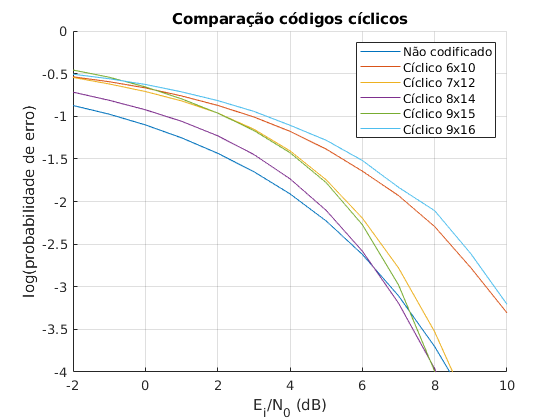
\includegraphics[scale=0.45]{floats/cyclic.png}
	\caption{\label{fig:cyclic}Comparação da eficácia dos códigos cíclicos para 96768 bits de informação enviados.}
\end{figure}

A Figura \ref{fig:proprios} mostra uma comparação entre todos os códigos desenvolvidos pela equipe na primeira prática.

\begin{figure}[ht]
	\centering
	\captionsetup{justification=centering}
	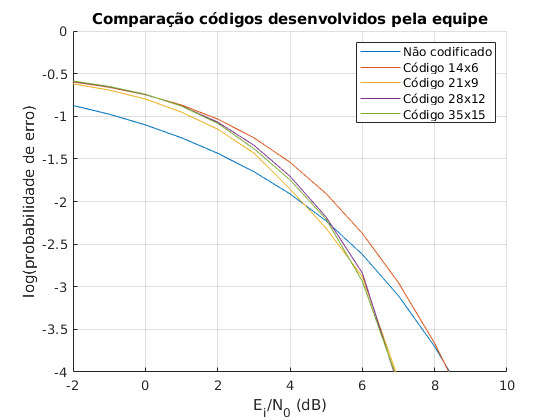
\includegraphics[scale=0.45]{floats/proprios.png}
	\caption{\label{fig:proprios}Comparação da eficácia dos códigos desenvolvidos pela equipe para 96768 bits de informação enviados.}
\end{figure}

As Figuras \ref{fig:convolucionais1}, \ref{fig:convolucionais2}, e \ref{fig:convolucionais3} mostram uma comparação entre todos os códigos convolucionais com as métricas de Hamming, Exata e distância Euclidiana respectivamente. A taxa para todos é $\frac{1}{3}$ e os polinômios utilizados são os do roteiro numerados na ordem em que aparecem no roteiro.

\begin{figure}[ht]
	\centering
	\captionsetup{justification=centering}
	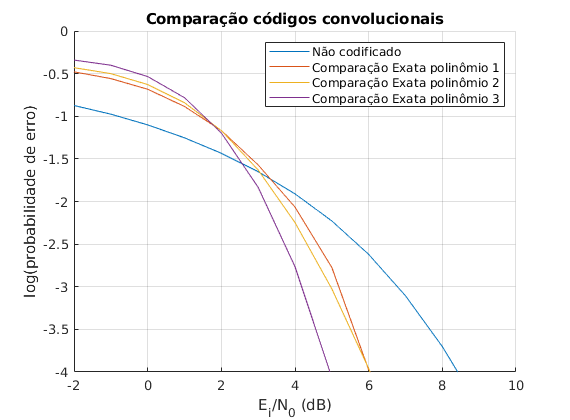
\includegraphics[scale=0.45]{floats/conv2.png}
	\caption{\label{fig:convolucionais2}Comparação da eficácia dos códigos convolucionais com distância 'Exata' para 96768 bits de informação enviados.}
\end{figure}


%
%\subsection{Códigos cíclicos não-BCH}
%
%\subsubsection{Polinômios geradores e distâncias mínimas}
%Os polinômios geradores utilizados e suas respectivas distâncias mínimas de código associado são mostradas em Listagem \ref{lst:polinomios}. Os índices são os mesmos do conjunto $S$ apresentado junto ao algoritmo. As distâncias mínimas, com mesma indexação de $S$, foram $\{2, 4, 3, 4, 2\}$.
%
%\begin{align}
%	\nonumber
%	p_1 = D^4+D^3+D^2+D+1\\ \nonumber
%	p_2 = D^5+D^3+D^2+1\\ \nonumber
%	p_3 = D^6+D^2+1\\ \nonumber
%	p_4 = D^6+D^4+D^3+D^2+1\\
%	p_5 = D^7+D^6+D^5+D^4+D^3+D^2+D+1
%	\label{lst:polinomios}
%\end{align}
%
%\subsubsection{Desempenho dos códigos cíclicos}
%
%Um gráfico comparativo entre os códigos aqui desenvolvidos e o código de Hamming é mostrado na Figura \ref{fig:cyclic_comparison}
%
%\begin{figure}[!hb]
%	\centering
%	\captionsetup{justification=centering}
%	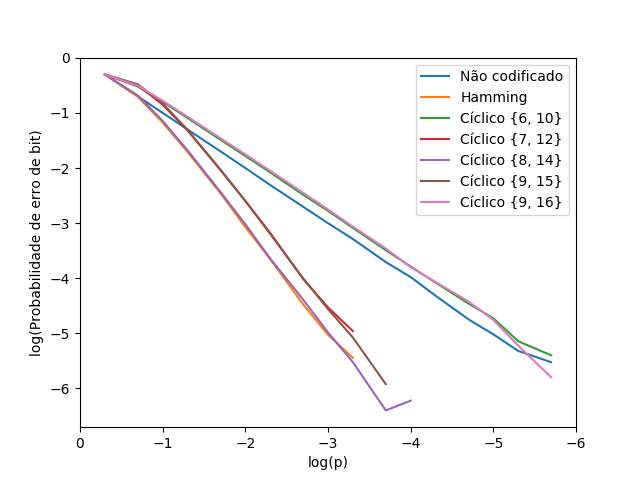
\includegraphics[scale=0.6]{floats/cyclic_5x10e6.png}
%	\caption{\label{fig:cyclic_comparison}Comparação da eficácia dos códigos cíclicos para 5004720 bits de informação enviados.}
%\end{figure}
%
%A título de comparação, a Figura \ref{fig:non_cyclic_comparison} traz os resultados do experimento anterior, o qual empregou códigos não necessariamente cíclicos obtidos pela tentativa de maximizar a distância mínima por meio de incrementos no tamanho de bloco.
%
%\begin{figure}[!hb]
%	\centering
%	\captionsetup{justification=centering}
%	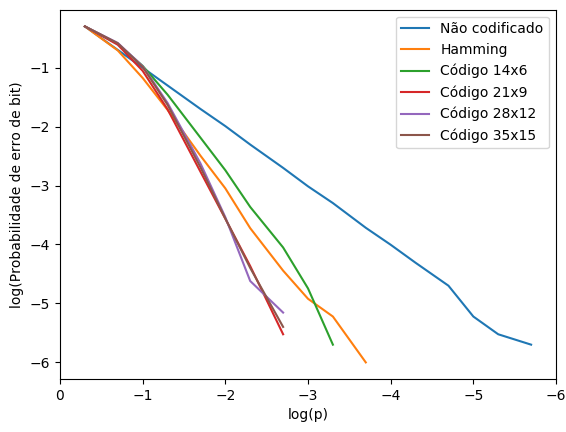
\includegraphics[scale=0.45]{floats/non_cyclic.png}
%	\caption{\label{fig:non_cyclic_comparison}Comparação da eficácia dos códigos não necessariamente cíclicos para 1000080 bits de informação enviados.}
%\end{figure}
%
%\subsection{Códigos BCH}
%
%\subsubsection{\label{complexidade_decod}Complexidade de decodificação BCH}
%
%Segundo \cite{ref:algoritmo-berlekamp}, a decodificação de códigos BCH se dá em $\mathcal{O}(n)$, $n$ sendo o tamanho de bloco empregado. Para confirmar a validade dessa afirmação, construíram-se códigos $BCH(m, 3)$, com $m \in \lbrace 4,5,...,20 \rbrace$, e mediram-se os tempos de decodificação submetendo a mesma palavra a cada um deles, com resultados ilustrados pela Figura \ref{fig:bch_decoding_is_linear}.
%
%\begin{figure}[!hb]
%	\centering
%    \captionsetup{justification=centering}
%	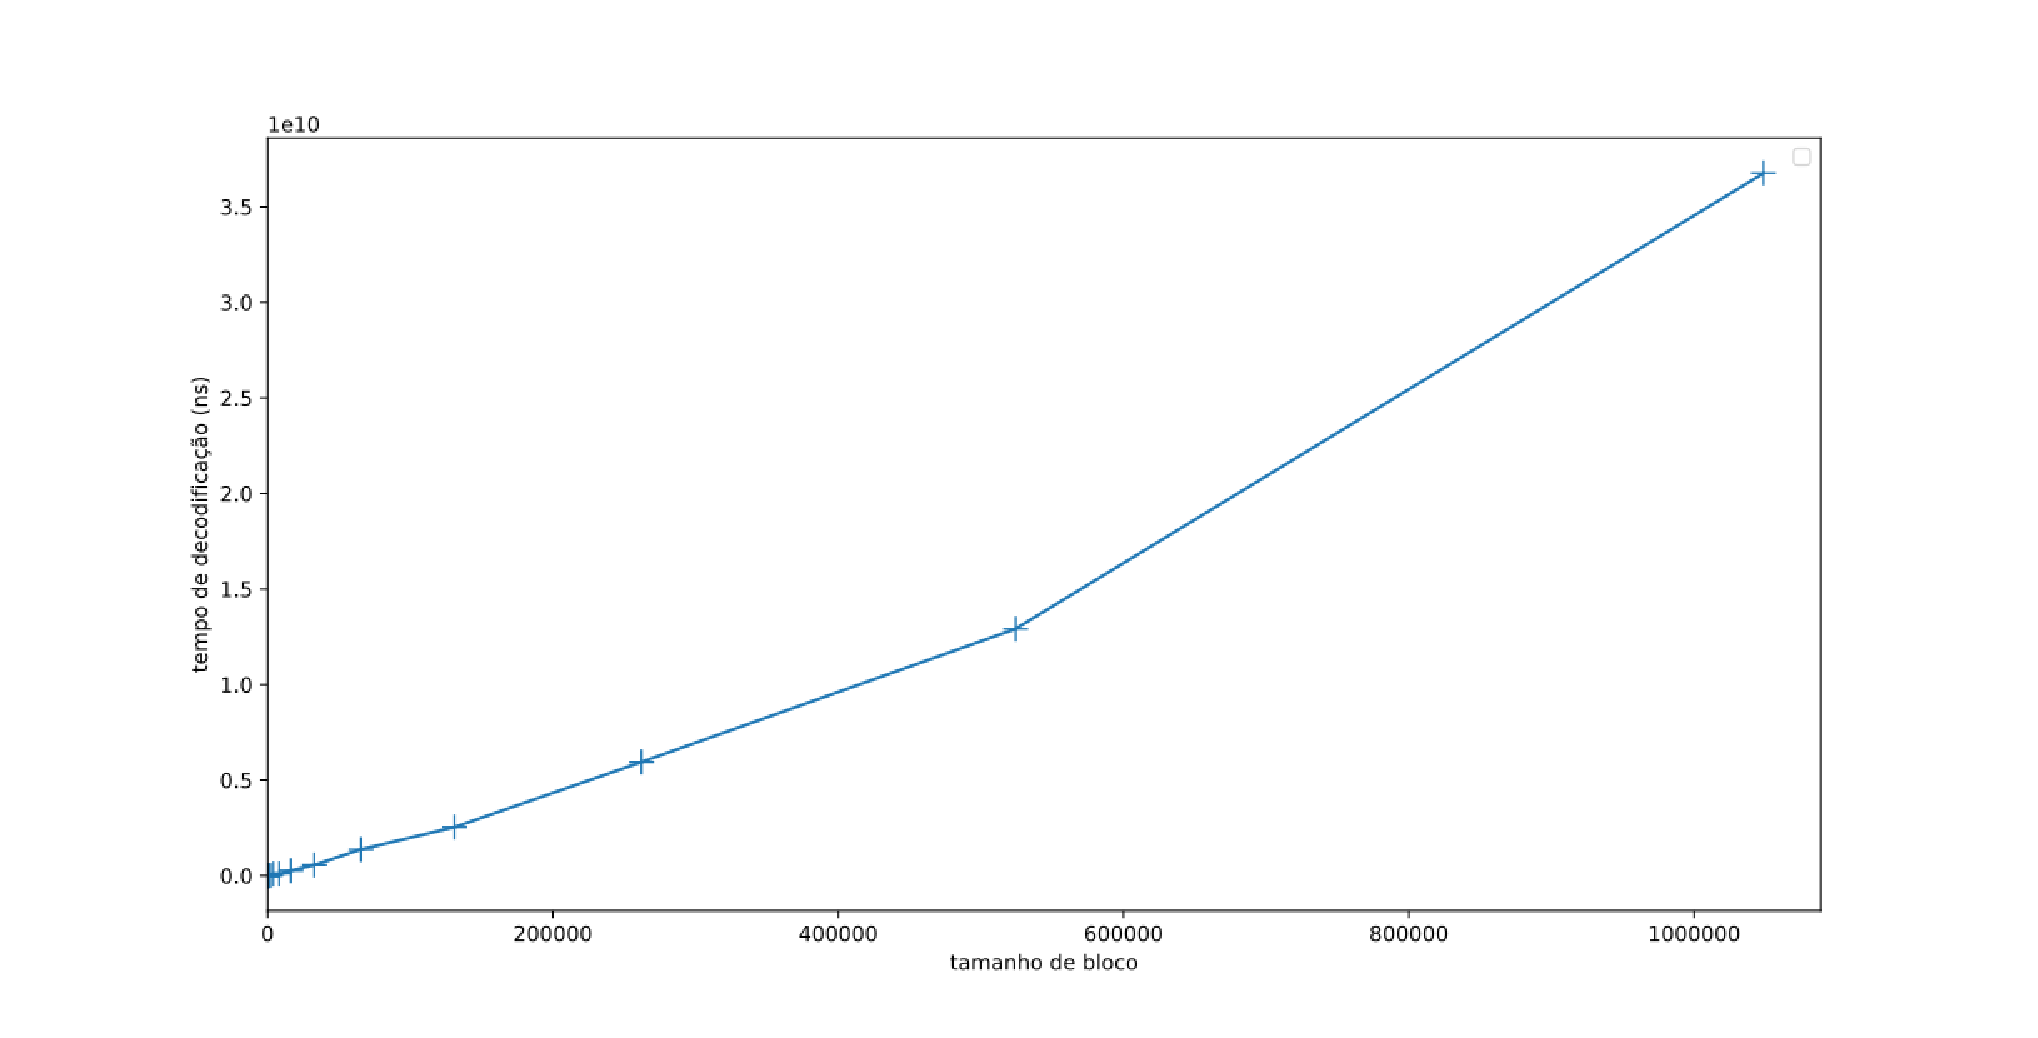
\includegraphics[scale=0.3]{floats/bch-decode-is-linear.eps}
%	\caption{\label{fig:bch_decoding_is_linear}Tempo de decodificação para BCH com variados tamanhos de bloco.}
%\end{figure}
%
%\subsubsection{\label{desempenho_bch}Desempenho do BCH}
%
%Para comparar o código BCH aos outros cíclicos, procurou-se um BCH de taxa próxima a 4/7 (usada como referência nos outros códigos deste laboratório), elegendo-se $BCH(5, 3)$ para ser submetido a testes sob canal BSC. A escolha se deu com base no polinômio gerador calculado, $g(X)=X^{15}+X^{11}+X^{10}+X^9+X^8+X^7+X^5+X^3+X^2+X+1$, que rendeu ao código taxa $\frac{31-15}{31}\simeq 0.52\simeq \frac{4}{7}\simeq 0.57$.
%
%Somente pela superior distância mínima projetada (3), era de se esperar que $BCH(5,3)$ superasse todos os outros códigos descritos neste texto. Isso é corroborado pela Figura \ref{fig:bch_performance}, na qual se vê que ele supera $Hamming(4,7)$ (que, por sua vez, tinha o mesmo desempenho aproximado dos outros códigos cíclicos).
%
%\begin{figure}[!hb]
%	\centering
%    \captionsetup{justification=centering}
%	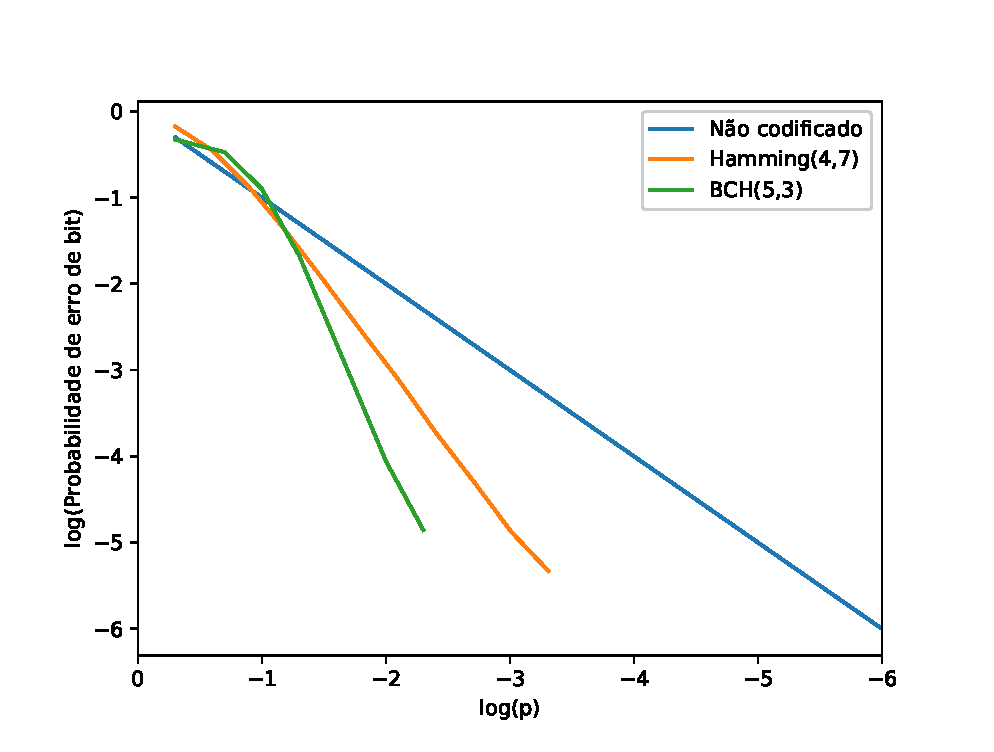
\includegraphics[scale=0.6]{floats/bch-performance.eps}
%	\caption{\label{fig:bch_performance}Chances de erro de bit de informação para $BCH(5,3)$ e $Hamming(4,7)$ sujeitos a canais BSC de variadas taxas de erro de bit.}
%\end{figure}

\section{Conclusão}

A maior dificuldade da implementação do codificador foi conseguir gerar o diagrama de transição de estados para efetuar o processamento da maquina, uma vez que realizar a convolução de sinais discretos possui um custo computacional mais elevado que cresce de acordo com o tamanho da mensagem.

Para o decodificador o maior desafio foi a implementação do algoritmo de Viterbi, uma vez que na primeira versão do código um pequeno detalhe de implementação gerou resultados errados retardando o desenvolvimento do decodificador. Outra dificuldade foi, no momento da implementação das variações, a implementação da segunda variação uma vez que foi necessário alterar o canal e alguns trechos do código foram alterados para operar com variáveis de ponto flutuante.

\begin{thebibliography}{1}

\bibitem{ref:algoritmo-berlekamp}
Berlekamp, Elwyn R. \emph{Algebraic Coding Theory}. Edição revisada. Singapura: WSPC, 2015. 
\bibitem{ref:roteiro}
Sharma, Manish \emph{Aula2 - Códigos Cíclicos}. ELE32-Introdução a Comunicações. 2018. 

\end{thebibliography}

\end{document}
